\chapter{Background}
\label{chapter:background}
% teaching the audience the tools they need to follow our work, because we use those tools

This chapter will introduce the essential concepts that underpin our work, which will be mentioned and utilized in subsequent chapters. 

\section{Classification in Machine Learning}

% paraphrase from https://towardsdatascience.com/machine-learning-classifiers-a5cc4e1b0623 
Classification is the process of determining the class of data points that have been provided. Classes are often referred to as targets/labels or categories. Predictive modeling for classification is the process of estimating a mapping function (f) from input variables (X) to discrete output variables (y). 

For instance, spam detection in email service providers can be considered a classification topic. This is a binary classification, as there are only two classes: spam and not spam. A classifier makes use of training data to examine the relation between provided input variables and the class. In this situation, training data must include both confirmed spam and non-spam emails. When the classifier is properly trained, it will be used to evaluate unknown emails. 

Classification is a type of supervised learning in which labels are available together with input data. It is applied in many industrial areas like target marketing, credit approval, medical diagnosis etc.

\section{Time Series Data}

% paraphrase from https://www.influxdata.com/what-is-time-series-data/ head lines
Time series data, often known as time-stamped data, is a collection of data points that are indexed chronologically. At different points in time, time-stamped data is collected. These data points are often composed of sequential measurements taken from the same source over a specified time interval and are used to monitor change over time. 

% paraphrase from https://www.investopedia.com/terms/t/timeseries.asp
Time series analysis may be beneficial for determining the evolution of an asset, security, or economic characteristic through time. More often, it can be used to examine how the changes related to the selected data point compare to shifts in other variables over the same timespan. 

Time series forecasting makes predictions about future activity by analyzing historical values and associated patterns. Typically, this is in reference to trend analysis, cyclical fluctuation analysis, and seasonality issues. As is the case with all forecasting techniques, success is not assured. 


\section{Semi-supervised Learning}

% paraphrase from https://bdtechtalks.com/2021/01/04/semi-supervised-machine-learning/
Only labeled samples are needed for supervised machine learning tasks, in which the model's ground truth must be specified during training.
Image classification, facial recognition, sales forecasting, customer churn prediction, and spam detection are all examples of supervised learning problems. 

Unsupervised learning, on the other hand, is used when the ground truth is unknown and machine learning models are applied to discover patterns in data. Customer segmentation, anomaly detection in network traffic, and content recommendation are all examples of unsupervised learning. 

Semi-supervised learning is a hybrid of the two. It handles classification issues, which means the task will eventually require a supervised learning method. At the same time, training the model without labeling each training sample, which unsupervised machine learning approaches may help with, is also incorporated. 

\section{Residual Neural Network}
ResNet~\cite{he2016deep} established the Residual Network idea to overcome the problem of the vanishing/exploding gradient.
This network employs a method known as skip connections.
The skip connection bypasses a few layers of training and links straight to the output. 
Instead of having layers learn the underlying mapping, this network is designed to suit the residual mapping.
Therefore, instead of stating $H(x)$, the initial mapping, let the network fit, $F(x):= H(x) - x$, which results in $H(x):= F(x) + x$. 

\begin{figure}[htbp!]
\centering
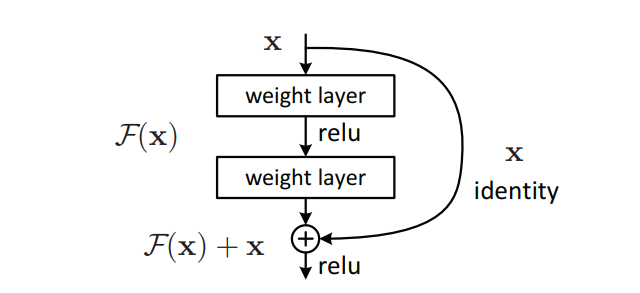
\includegraphics[width=0.5\textwidth]{images/background/Residual-Block.PNG}
\caption{Skip (Shortcut) connection}
\label{fig:res_block}
\end{figure}

The benefit of introducing this sort of skip connection is that if any layer hinders the efficiency of the architecture, then regularization will skip it.
As a result, extremely deep neural networks may be trained without the issues caused by vanishing/exploding gradients. 

\section{Pooling}

Pooling in convolutional neural networks is a technique for generalizing features extracted by convolutional filters and helping the network recognize features independent of their positions in the image. 

The fundamental process of pooling closely resembles that of convolution. Choose a filter and slide it over the output feature map of the preceding convolutional layer. The most prevalent filter size is 2x2, and it is slid over the input using a stride of 2. The pooling filter calculates an output on the receptive field (the part of the feature map under the filter) based on the specified type of pooling operation. 

By using pooling, we extract the feature into a smaller, more generic map that displays merely the presence or absence of a feature in each quadrant. With each succeeding layer, the map becomes more compact, retaining only the essential information on the existence of the features of interest. As the map gets smaller, it becomes increasingly independent of the location of the feature. As long as the feature has been identified in the general vicinity of the original location, it should appear similarly in the map created by the pooling layers. 

% to add
\section{Evaluation Metrics}

After doing the standard feature engineering, selection, and implementation of a model and obtaining some output in the form of a probability or a class, the next step is to find out how effective is the model based on some certain metrics using test datasets. Metrics for evaluating the machine learning model are crucial. Choice of metrics influences how the performance of machine learning algorithms is measured and compared. For now, the focus is on the ones used for Classification problems.


\subsection{AUC}

\begin{figure}[htbp!]
\centering
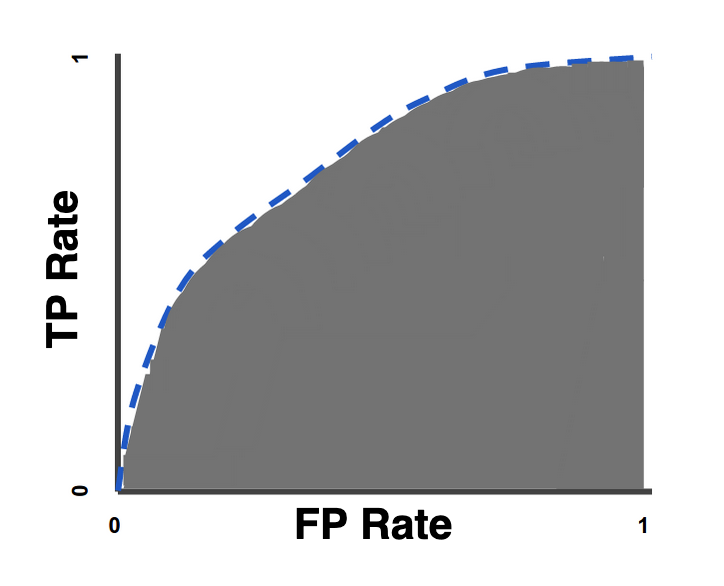
\includegraphics[width=0.5\textwidth]{images/background/auc_roc.png}
\caption{AUC (Area Under the ROC Curve)}
\label{fig:roc_auc}
\end{figure}


The AUC - ROC curve is a performance metric for classifying issues using a variety of threshold values. The receiver operating characteristic (ROC) curve is a probability curve, and the area under the curve (AUC) represents the degree or measure of separability. AUC is the abbreviation for "Area under the ROC Curve." That is, AUC quantifies the full two-dimensional area beneath the entire ROC curve from (0,0) to (1,1). AUC is a measure of performance that is aggregated across all feasible classification thresholds. 

AUC may be interpreted in several ways. One method is to think of it as the likelihood that the model would rank a random positive example higher than a random negative example. It indicates the degree to which the model is capable of differentiating between classes. The greater the AUC value, the more accurately the model predicts 0 classes as 0 and 1 classes as 1. 

\subsection{F1 Score}

Precision and recall are the two most often used criteria for assessing class imbalance.Additionally, they serve as the foundation for the F1 score. 
\paragraph{Precision}
Precision attempts to quantify What proportion of positive identifications was actually correct. It is defined as follows:
\[\text{Precision} = \frac{\text{TP}}{\text{TP} + \text{FP}}\]

\paragraph{Recall}
Recall attempts to quantify What proportion of actual positives was identified correctly. It is defined as follows:
\[\text{Recall} = \frac{\text{TP}}{\text{TP} + \text{FN}}\]



\paragraph{F1}
The F1 score's objective is to merge precision and recall into a single metric. Meanwhile, the F1 score has been designed to perform well on imbalanced data. 
The F1 score is defined as the harmonic mean of precision and recall. The F1 score is computed by averaging accuracy and recall. They are both rates, which makes  the harmonic mean the reasonable choice. The F1 score formula is shown as below:
\[F_{1}=2 * \frac{\text{Precision} * \text{Recall}}{\text{Precision} + \text{Recall}}\]


% \section{LSTM cell}







































% % to use as basis for explanation

% \subsection{Learned Sketch}

% \begin{figure}[htbp!]
% 	\centering
% 	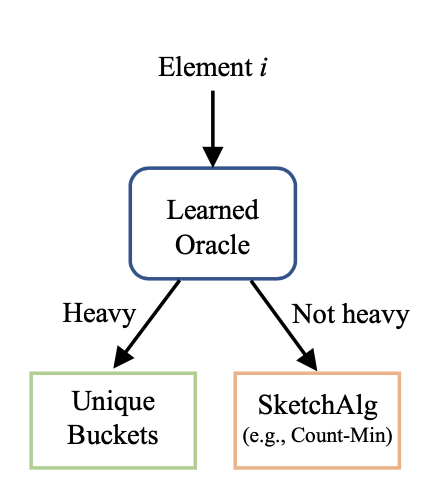
\includegraphics[width=0.5\linewidth]{images/plots/NN_Sketch.png}
% 	\caption{Learn Sketch diagram}
% 	\label{fig:NN+Sketch}
% \end{figure}

% This diagram shows the full system, i.e., the system is composed of Learned Oracle, Unique Buckets and Sketch Algorithm.
% % from Learn Sketch